\scanpage{43}
with the torsor $P_s$ under $G_{k(s)}$ and the trivialization $p(x)\in P_s(\mathbb{C})$.

In terms of $\unsure{w|\omega}$ and $q:\bar S_{\mathbb{C}}\longrightarrow P_{\mathbb{C}}^{\mathrm{an}}$, giving $f$ amounts to giving
\[
f:\bar S_{\mathbb{C}}\longrightarrow\unsure{\gamma|\mathscr{Y}}_G
\]
satisfying the conditions

a) $f$ holomorphic

b) $f(xg)=w(g)^{-1}f(x)$

c) \deleted{$\unsure{f(\xi_0)|f(\bar\xi_0)}$} $\forall\bar s\in\bar S_{\mathbb{C}}$, \inserted{over $s\in S$} $f(\bar s):\mathbb{S}\relbarG_{\mathbb{R}}$ is compatible with the torsor $P_s$ over $G_{k(s)}$ and its trivialization $q(x)\in P_s(\mathbb{C})$.

Finally, \deleted{for every $k$}, we are given a ``\unsure{restriction|restriction}'' of the covering $\widetilde{\mathbb P}_{\mathbb{C}}\mathbin{\times}^{G(\mathbb{Q})}G(\mathcal A)\deleted{\mathbb{Q}_{\ell}}$ over $S_{\mathbb{C}}^{\mathrm{an}}$ to a covering
% slanted
\margin{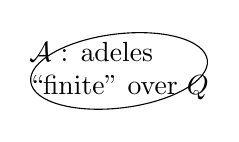
\begin{tikzpicture}[baseline=(current bounding box.center)]
\node[inner sep=0pt,align=left] (note) {$\mathcal A$ : adeles\\``finite'' over $\mathbb{Q}$};
\draw[rotate around={7:(note.center)}] (note.center) ellipse [x radius=1.13cm,y radius=.47cm];
\end{tikzpicture}}
\deleted{over $S$ of which of \unsure{group|group} $G_\ell$} of group $G(\mathbb{Q}_{\ell})$ over $S$, In terms \inserted{of $\xi_0$ and} of $\Gamma=\pi_1(S(\mathbb{C}),\unsure{\xi|\mathord{)}}_0)$, we are given a factorization of $\Gamma\xrightarrow{w}G(\mathbb{Q})\relbarG(\mathcal A)$ through $\Gamma\longrightarrow\Pi_1\underset{\substack{\Vert\\\Pi_1}}{(S},\xi_0)\longrightarrow G(\mathcal A)$. As for the covering $\widetilde P_{\mathbb{C}}\mathbin{\times}^{G(\mathbb{Q})}(\deleted{\unsure{G|\mathcal A}}\mathcal A/G^{\unsure{0|\circ}})(\mathcal A)$, \deleted{equal to $\widetilde P_{\mathbb{C}}\times$}\inserted{it is} associated to $\widetilde P_{\mathbb{C}}/G^0(\mathbb{Q})\deleted{\text{of}}\unsure{=|\relbar}(P/G^0)_{\mathbb{C}}^{\mathrm{an}}$, \deleted{\unsure{which|which}}and \unsure{as|:} such \unsure{their|their} restriction to $S$ \deleted{\unsure{is|and}} is known. We want these to be those given above.....

\deleted{\uline{NB} \unsure{The map|the map} $f$ \unsure{is|and}}
% archive sheet number: 42
